\documentclass[pdftex,10pt,xcolor=svgnames]{beamer}

\mode<presentation>
{
  \usetheme{boxes}
  \usecolortheme[named=MidnightBlue]{structure}
  %\setbeamercolor{normal text}{bg=NavajoWhite!20}
  \usefonttheme{serif}
  \setbeamertemplate{navigation symbols}{}
  % Show frame number and author name in footline
  \setbeamertemplate{footline}[frame number]
  \addtobeamertemplate{footline}{\quad\textcolor{gray}{David Duvenaud and James Lloyd}}{}
  % Set frame titles in small capitals
  \setbeamerfont{frametitle}{shape=\scshape,family=\rmfamily}
  \setbeamercolor{frametitle}{bg=gray!60!white,fg=black}
  % Alerted text: blue (uncomment second line if theme sets alerted text to bold)
  \setbeamercolor{alerted text}{fg=blue}
  %\setbeamerfont*{alerted text}{}
  \setbeamertemplate{bibliography item}[text] %{\hbox{\donotcoloroutermaths$\blacktriangleright$}}
  \setbeamertemplate{bibliography entry title}{}
  \setbeamertemplate{bibliography entry author}{}
  \setbeamertemplate{bibliography entry note}{}
  \setbeamertemplate{bibliography entry location}{}

}
\usepackage[english]{babel}
\usepackage[latin1]{inputenc}
\usepackage{times}
\usepackage[T1]{fontenc}
\usepackage{hyperref}
\usepackage{multimedia}
\usepackage{eepic}
\usepackage{graphicx}
%\usepackage[nohug]{latexinclude/diagrams}
\usepackage{tikz}
\usetikzlibrary{calc}

%% \newcommand{\footlineextra}[1]{
%%     \begin{tikzpicture}[remember picture,overlay]
%%         \node[yshift=1.5ex,anchor=south east] at (current page.south east)
%% {#1};
%%     \end{tikzpicture}
%% }

\newcommand{\footlineextra}[1]{
    \begin{tikzpicture}[remember picture,overlay]
        \node[xshift=-5ex,yshift=-0.5ex,anchor=south east] at (current page.south east)
             {\mbox{\tiny \textcolor{MidnightBlue}{#1}}};
    \end{tikzpicture}
}

\def\sectionframe#1{
  {
    \setbeamertemplate{footline}{\empty}
    \begin{frame}{}
      \begin{center}
        \huge\sc #1
      \end{center}
    \end{frame}
  }
}


\usepackage{listings}
%\usepackage[usenames,dvipsnames]{color}
% This is the color used for MATLAB comments below
\definecolor{MyDarkGreen}{rgb}{0.0,0.4,0.0}

% For faster processing, load Matlab syntax for listings
\lstloadlanguages{Matlab}%
\lstset{language=Matlab,                        % Use MATLAB
        frame=none,                           % Single frame around code
        basicstyle=\small\ttfamily,             % Use small true type font
        keywordstyle=[1]\color{Blue}\bf,        % MATLAB functions bold and blue
        keywordstyle=[2]\color{Purple},         % MATLAB function arguments purple
        keywordstyle=[3]\color{Blue}\underbar,  % User functions underlined and blue
        identifierstyle=,                       % Nothing special about identifiers
                                                % Comments small dark green courier
        commentstyle=\usefont{T1}{pcr}{m}{sl}\color{MyDarkGreen}\small,
        stringstyle=\color{Purple},             % Strings are purple
        showstringspaces=false,                 % Don't put marks in string spaces
        tabsize=5,                              % 5 spaces per tab
        %
        %%% Put standard MATLAB functions not included in the default
        %%% language here
        morekeywords={xlim,ylim,var,alpha,factorial,poissrnd,normpdf,normcdf},
        %
        %%% Put MATLAB function parameters here
        morekeywords=[2]{on, off, interp},
        %
        %%% Put user defined functions here
        morekeywords=[3]{FindESS, homework_example,randg},
        %
        morecomment=[l][\color{Blue}]{...},     % Line continuation (...) like blue comment
        numbers=left,                           % Line numbers on left
        firstnumber=1,                          % Line numbers start with line 1
        numberstyle=\tiny\color{Blue},          % Line numbers are blue
        stepnumber=1                            % Line numbers go in steps of 5
        }

% Includes a MATLAB script.
% The first parameter is the label, which also is the name of the script
%   without the .m.
% The second parameter is the optional caption.
\newcommand{\matlabscript}[2]
  {\begin{itemize}\item[]\lstinputlisting[caption=#2,label=#1]{#1.m}\end{itemize}}

\newcommand{\inputmatlab}[1]
  {\begin{lstlisting}[language=Matlab] \input{#1} \end{lstlisting}}



\usecolortheme{default}
% colours
\xdefinecolor{Black}{rgb}{0,0,0}
\xdefinecolor{White}{rgb}{1,1,1}
\xdefinecolor{DarkBlue}{rgb}{0,0,.7}
\xdefinecolor{DarkRed}{rgb}{.7,0,0}
\xdefinecolor{Red}{rgb}{.85,0,0}
\xdefinecolor{DarkGreen}{rgb}{0,.7,0}
\xdefinecolor{DarkMagenta}{rgb}{.6,0,.6}
\def\Black{\textcolor{Black}}
\def\White{\textcolor{White}}
\def\Blue{\textcolor{DarkBlue}}
\def\Magenta{\textcolor{DarkMagenta}}
\def\Red{\textcolor{Red}}
\def\Green{\textcolor{DarkGreen}}

\usepackage{alltt}
\usepackage{psfrag}
\usepackage{pstool}
\usepackage{ulem}
%\usepackage{listings}

\usepackage{picins}
\usepackage{tikz}
\usetikzlibrary{shapes.geometric,arrows,chains,matrix,positioning,scopes,calc}
\tikzstyle{mybox} = [draw=white, rectangle]

\title[] % (optional, use only with long paper titles)
{Introduction to probabilistic programming}

\author % (optional, use only with lots of authors)
{David Duvenaud and James Lloyd}
% - Use the \inst{?} command only if the authors have different
%   affiliation.

\institute[] % (optional, but mostly needed)
{University of Cambridge}
% - Use the \inst command only if there are several affiliations.
% - Keep it simple, no one is interested in your street address.

\date % (optional)
{\empty}

\subject{Talks}

\usetikzlibrary{shapes.geometric,arrows,chains,matrix,positioning,scopes}
 \makeatletter
 \tikzset{join/.code=\tikzset{after node path={%
       \ifx\tikzchainprevious\pgfutil@empty\else(\tikzchainprevious)%
       edge[every join]#1(\tikzchaincurrent)\fi}}
 }
 \tikzset{>=stealth',every on chain/.append style={join},
   every join/.style={->}
 }

\tikzstyle{mybox} = [draw=white, rectangle]
\usepackage{ifthen}
\usepackage{booktabs}

% Custom definitions
%\def\simiid{\sim_{\mbox{\tiny iid}}}
\def\simiid{\stackrel{\mathrm{iid}}{\sim}}

%%%%%%%%%%%%%%%%%%%%%%%%%%%%%%%%%%%%%%%%%%%%%%%%%%%%%%%%%%
%%%% EDITING HELPER FUNCTIONS  %%%%%%%%%%%%%%%%%%%%%%%%%%%
%%%%%%%%%%%%%%%%%%%%%%%%%%%%%%%%%%%%%%%%%%%%%%%%%%%%%%%%%%

%% NA: needs attention (rough writing whose correctness needs to be verified)
%% TBD: instructions for how to fix a gap ("Describe the propagation by ...")
%% PROBLEM: bug or missing crucial bit 

%% use \fXXX versions of these macros to put additional explanation into a footnote.  
%% The idea is that we don't want to interrupt the flow of the paper or make it 
%% impossible to read because there are a bunch of comments.

%% NA's (and TBDs, those less crucially) should be written so 
%% that they flow with the text.

\definecolor{WowColor}{rgb}{.75,0,.75}
\definecolor{SubtleColor}{rgb}{0,0,.50}

% inline
\newcommand{\NA}[1]{\textcolor{SubtleColor}{ {\tiny \bf ($\star$)} #1}}
\newcommand{\LATER}[1]{\textcolor{SubtleColor}{ {\tiny \bf ($\dagger$)} #1}}
\newcommand{\TBD}[1]{\textcolor{SubtleColor}{ {\tiny \bf (!)} #1}}
\newcommand{\PROBLEM}[1]{\textcolor{WowColor}{ {\bf (!!)} {\bf #1}}}

% as margin notes

\newcounter{margincounter}
\newcommand{\displaycounter}{{\arabic{margincounter}}}
\newcommand{\incdisplaycounter}{{\stepcounter{margincounter}\arabic{margincounter}}}

\newcommand{\fTBD}[1]{\textcolor{SubtleColor}{$\,^{(\incdisplaycounter)}$}\marginpar{\tiny\textcolor{SubtleColor}{ {\tiny $(\displaycounter)$} #1}}}

\newcommand{\fPROBLEM}[1]{\textcolor{WowColor}{$\,^{((\incdisplaycounter))}$}\marginpar{\tiny\textcolor{WowColor}{ {\bf $\mathbf{((\displaycounter))}$} {\bf #1}}}}

\newcommand{\fLATER}[1]{\textcolor{SubtleColor}{$\,^{(\incdisplaycounter\dagger)}$}\marginpar{\tiny\textcolor{SubtleColor}{ {\tiny $(\displaycounter\dagger)$} #1}}}


%% For submission, make all render blank.
%\renewcommand{\LATER}[1]{}
%\renewcommand{\fLATER}[1]{}
%\renewcommand{\TBD}[1]{}
%\renewcommand{\fTBD}[1]{}
%\renewcommand{\PROBLEM}[1]{}
%\renewcommand{\fPROBLEM}[1]{}
%\renewcommand{\NA}[1]{#1}  %% Note, NA's pass through!

\begin{document}

\small

%% { 
%%   \setbeamertemplate{footline}{\empty}
%%   \begin{frame}
%%     \titlepage
%%   \end{frame}
%% }
\renewcommand{\inserttotalframenumber}{11}

\theoremstyle{plain}

\def\ie{i.e.\ }
\def\eg{e.g.\ }
\def\indicator{\mathbb{I}}
\def\mean#1{\mathbb{E}[#1]}
\def\bigmean#1{\mathbb{E}\bigl[#1\bigr]}
\def\Bigmean#1{\mathbb{E}\Bigl[#1\Bigr]}
\def\cyl{\mathcal{Z}}
\def\eqae{=_{\mbox{\tiny a.e.}}}
\def\wrt{w.r.t.\ }
\def\ae{a.e.\ }
\def\equas{=_{\mbox{\tiny a.s.}}}
\def\equae{=_{\mbox{\tiny a.e.}}}
\def\iid{i.i.d.\ }
\def\Iid{I.i.d.\ }
%\def\inclusion{\jmath}
\def\inclusion{\mathcal{J}}
\def\inclusionX{\inclusion_{\xspace}}
\def\wstar{weak$^{\ast}$ }
% Symmetric difference
\def\symmdiff{\!\vartriangle\!}


% Indices

\def\indI{\mbox{\tiny I}}
\def\indJ{\mbox{\tiny J}}
\def\indK{\mbox{\tiny K}}
\def\indJI{\mbox{\tiny J$\setminus$I}}
\def\indE{\mbox{\tiny E}}
\def\indF{\mbox{\tiny F}}
\def\indD{\mbox{\tiny D}}
\def\indi{\mbox{\tiny{\{i\}}}}
\def\ind#1{\mbox{\tiny #1}}
\def\power{\mathcal{F}}
\def\powerD{\power(D)}
\def\powerE{\power(E)}
\def\powerL{\power(L)}
\def\parts{\mathcal{H}}
\def\partsQ{\parts(\mathcal{Q})}
\def\partsn{\parts[n]}
\def\partsN{\parts_{\infty}(\mathbb{N})}

% Spaces

\def\abstspace{\Omega}
\def\xspace{\mathcal{X}}
\def\yspace{\mathcal{Y}}
\def\tspace{\mathcal{T}}
\def\xspaceI{\xspace_{\indI}}
\def\xspaceJ{\xspace_{\indJ}}
\def\xspaceD{\xspace_{\indD}}
\def\xspaceE{\xspace_{\indE}}
\def\tspaceI{\tspace_{\indI}}
\def\tspaceJ{\tspace_{\indJ}}
\def\tspaceD{\tspace_{\indD}}
\def\tspaceE{\tspace_{\indE}}
\def\txspace{\tilde{\xspace}}
\def\yspaceI{\yspace_{\indI}}
\def\yspaceJ{\yspace_{\indJ}}
\def\yspaceD{\yspace_{\indD}}
\def\yspaceE{\yspace_{\indE}}
\def\txspace{\tilde{\xspace}}
\def\ttspace{\tilde{\tspace}}
\def\xI{x_{\indI}}
\def\xJ{x_{\indJ}}
\def\xD{x_{\indD}}
\def\xE{x_{\indE}}
\def\tImage{\Gamma}
\def\simp{\triangle}
\def\simpI{\simp_{\indI}}
\def\simpJ{\simp_{\indJ}}

\def\AI{A_{\indI}}
\def\AJ{A_{\indJ}}
\def\AD{A_{\indD}}
\def\AE{A_{\indE}}


%Space of Prob Measures
\def\pMeas{M}
%Space of Contents
\def\fMeas{N}
%Space of cont fcts
\def\cfspace{C}
%Hilbert space
\def\hilbert{\mathcal{L}^2}


\def\borelV{\borel_{V}}

% Set systems

\def\borel{\mathcal{B}}
\def\top{\mbox{Top}}

\def\borelI{\borel_{\indI}}
\def\borelJ{\borel_{\indJ}}
\def\borelD{\borel_{\indD}}
\def\borelE{\borel_{\indE}}
\def\tborel{\tilde{\borel}}
\def\abstfield{\mathcal{A}}
\def\field{\mathcal{C}}
\def\fieldI{\field_{\indI}}
\def\fieldJ{\field_{\indJ}}
\def\fieldK{\field_{\indK}}
\def\fieldD{\field_{\indD}}
\def\fieldE{\field_{\indE}}
\def\tfield{\tilde{\mathcal{C}}}
\def\Sfield{\mathcal{S}}
\def\SfieldI{\mathcal{S}_{\indI}}
\def\SfieldJ{\mathcal{S}_{\indJ}}
\def\SfieldD{\mathcal{S}_{\indD}}
\def\tSfield{\tilde{\mathcal{S}}}
\def\borelx{\borel_x}
\def\tborelx{\tborel_x}
\def\borelgamma{\tborel_{\tImage}}
%\def\borelth{\borel_{\theta}}
\def\borely{\borel_{y}}
%\def\borelT{\borel_t}
\def\borelT{\borel_{\tspace}}
\def\borelS{\borel_s}
\def\topI{\top_{\indI}}
\def\topJ{\top_{\indJ}}
\def\topD{\top_{\indD}}
\def\topE{\top_{\indE}}
\def\topV{\top_V}
\def\topws{\top_{\text{ws}}}
\def\topcc{\top_{\text{c}}}
\def\borelXI{\borel(\xspaceI)}
\def\borelXD{\borel(\xspaceD)}
\def\tborelX{\borel(\txspace)}
\def\borelTI{\borel(\tspaceI)}
\def\borelTD{\borel(\tspaceD)}
\def\tborelT{\borel(\ttspace)}


% Maps

\def\XI{X_{\indI}}
\def\Xi{X_{\ind{i}}}
\def\Xj{X_{\ind{j}}}
\def\ThetaI{\Theta_{\indI}}
\def\XJ{X_{\indJ}}
\def\ThetaJ{\Theta_{\indJ}}
\def\XD{X_{\indD}}
\def\ThetaD{\Theta_{\indD}}
\def\XE{X_{\indE}}
\def\ThetaE{\Theta_{\indE}}
\def\tX{\tilde{X}}
\def\tTheta{\tilde{\Theta}}

\def\SI{S_{\indI}}
\def\TI{T_{\indI}}

\def\rest{\phi}
\def\restD{\rest_{\indD}}
\def\restI{\rest_{\indI}}
\def\restJ{\rest_{\indJ}}
\def\restDI{\rest^{\indD}_{\indI}}
\def\inclusionD{\inclusion_{\indD}}
\def\inclusionE{\inclusion_{\indE}}
\def\projector{\mbox{pr}}
\def\projectorD{\projector_{\indD}}
\def\projectorI{\projector_{\indI}}
\def\projectorJI{\pi_{\indJ\indI}}
\def\indicator{\mathbb{I}}

% Projective systems

\def\po{\preceq}
\def\famD#1{{\lbrace #1 \rbrace}_{\indD}}
\def\famE#1{{\lbrace #1 \rbrace}_{\ind{I$\in$}\indE}}
\def\fJI{f_{\indJ\indI}}
\def\fKI{f_{\indK\indI}}
\def\fKJ{f_{\indK\indJ}}
\def\fII{f_{\indI\indI}}
\def\fI{f_{\indI}}
\def\fJ{f_{\indJ}}
\def\fK{f_{\indK}}
\def\fD{f_{\indD}}
\def\fDI{f^{\indD}_{\indI}}
\def\fDK{f^{\indD}_{\indK}}
\def\gJI{g_{\indJ\indI}}
\def\gI{g_{\indI}}
\def\gJ{g_{\indJ}}
\def\gD{g_{\indD}}
\def\hJI{h_{\indJ\indI}}
\def\hI{h_{\indI}}
\def\hJ{h_{\indJ}}
\def\hE{h_{\indE}}
\def\plim{\varprojlim}

% Measure and Conditionals

\def\abstmeasure{\mathbb{P}}
\def\P{P}
\def\PI{P_{\indI}}
\def\PJ{P_{\indJ}}
\def\PD{P_{\indD}}
\def\PE{P_{\indE}}
\def\PX{P_{\mbox{X}}}
\def\PTh{P_{\mbox{\Theta}}}
\def\PXI{P_{\XI}}
\def\PThI{P_{\mbox{\Theta}}}
\def\PXJ{P_{\mbox{X}}}
\def\PThJ{P_{\mbox{\Theta}}}
\def\PXD{P_{\mbox{X}}}
\def\PThD{P_{\mbox{\Theta}}}
\def\PXE{P_{\mbox{X}}}
\def\PThE{P_{\mbox{\Theta}}}
\def\tP{\tilde{P}}
\def\tPX{\tilde{P}_X}
\def\tPTh{\tilde{P}_{\Theta}}







\def\SI{S_{\indI}}
\def\SJ{S_{\indJ}}

\def\tk{\tilde{k}}
\def\kI{k_{\indI}}

\def\postkernel{k}
\def\indctr{\mathbbm{1}}
\def\sp#1{\left<#1\right>}


%Mallows
\def\Sr{\mathbb{S}_r}
\def\Sinf{\mathbb{S}_{\infty}}
\def\Sbar{\bar{\mathbb{S}}}
\def\DP#1{\mbox{DP}\left( #1 \right)}
\def\GP#1{\mbox{GP}\left( #1 \right)}
\def\x{\mathbf{x}}
\def\y{\mathbf{y}}



\def\tyspace{\tilde{\yspace}}
\def\tF{\tilde{F}}
\def\tT{\tilde{T}}
\def\tmodel{\tilde{\model}}
\def\tnu{\tilde{\nu}}


\def\PTheta{P^{\theta}}
\def\FTheta{F^{\theta}}
\def\TTheta{T^{\theta}}
\def\borelY{\borel_{\yspace}}

\def\PX{P^{x}}
\def\PXI{\PX_{\indI}}
\def\PXJ{\PX_{\indJ}}
\def\PXD{\PX_{\indD}}
\def\PThetaI{\PTheta_{\indI}}
\def\PThetaD{\PTheta_{\indD}}
\def\YI{Y_{\indI}}
\def\YJ{Y_{\indJ}}
\def\YD{Y_{\indD}}
\def\Tn{T^{(n)}}
\def\indexspace{\mathcal{W}}
\def\tyspace{\tilde{\yspace}}
\def\tY{\tilde{Y}}
\def\inclusionT{\inclusion_{\tspace}}
\def\tPTheta{\tilde{P}^{\theta}}
\def\tTn{\tilde{T}^{(n)}}
\def\inclusionY{\inclusion_{\yspace}}

\def\tyspace{\tilde{\yspace}}
\def\tF{\tilde{F}}
\def\tT{\tilde{T}}
\def\tmodel{\tilde{\model}}
\def\tnu{\tilde{\nu}}
\def\tOmega{\tilde{\abstspace}}
\def\tabstmeasure{\tilde{\abstmeasure}}
\def\model{\mathcal{P}}

\def\tf{\tilde{f}}
\def\tx{\tilde{x}}
\def\Dom{\mbox{Dom}}
\def\ty{\tilde{y}}


\begin{frame}
  \begin{block}{}
    \titlepage
  \end{block}
  \begin{center}
    {\bf Thanks to}\\
    Daniel M Roy (Cambridge)\\
    Roger Grosse (MIT)
  \end{center}
\end{frame}

\begin{frame}{How to write a Bayesian modeling paper}
  \begin{block}{}
    \begin{enumerate}
      \item Write down a generative model in an afternoon
      \vspace{\baselineskip}
      \vspace{\baselineskip}
      \item Get 2 grad students to implement inference for a month
      \vspace{\baselineskip}
      \vspace{\baselineskip}
      \item Use technical details of inference to pad half of the paper
    \end{enumerate}
  \end{block}
\end{frame}

\begin{frame}{Can we do better?}
  \begin{block}{Example: Graphical Models}  
  \end{block}
      \begin{block}{Application Papers}
      \begin{enumerate}
        \item Write down a graphical model
        \item Perform inference using general-purpose software
        \item Apply to some new problem
      \end{enumerate}
    \end{block}
      \begin{block}{Inference papers}
      \begin{enumerate}
        \item Identify common structures in graphical models (e.g. chains)
        \item Develop efficient inference method
        \item Implement in a general-purpose software package
      \end{enumerate}
    \end{block}  
  \begin{block}{}
      \vspace{-2\baselineskip}
  \large
    \begin{center}
    {
      {Modeling and inference have been disentangled}
    }	
    \end{center}
  \end{block}
\end{frame}



\begin{frame}{Expressivity}
  \begin{block}{Not all models are graphical models}  
  What is the largest class of models available?
  \end{block}
  \vspace{\baselineskip}
  \begin{block}{Probabilistic Programs}
      \begin{itemize}
        \item A probabilistic program (PP) is any program that can depend on random choices.  Can be written in any language that has a random number generator.
        \item You can specify any (computable) prior by simply writing down a PP that generates samples
        \item Any PP implicitly defines a distribution over its output.
        \begin{itemize}
		     \item It also defines a distribution over \emph{execution traces}: the set of states the interpreter went through when running the program.
        \end{itemize}
      \end{itemize}
    \end{block}
\end{frame}

\begin{frame}{An Example Probabilistic Program}

%\begin{alltt}
\begin{lstlisting}[language=Matlab]
flip = rand < 0.5
if flip
    x = randg + 2   % Random draw from Gamma(1,1)
else
    x = randn       % Random draw from standard Normal
end
\end{lstlisting}
%\end{alltt}

\pause
  \begin{block}{Implied distributions over variables}

  %\begin{figure}
  \only<1-2>{
	  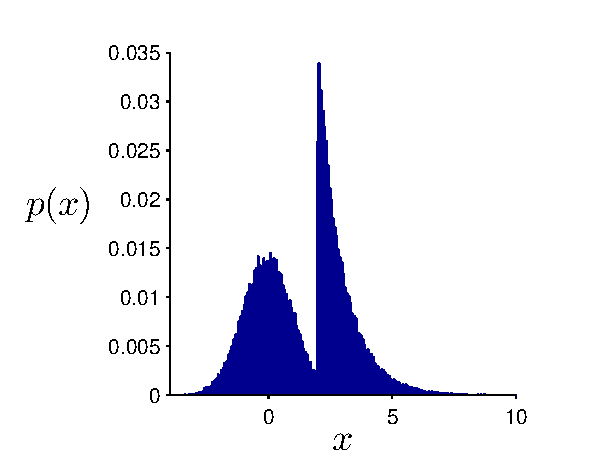
\includegraphics[width=0.45\textwidth]{figures/xmarg}
	  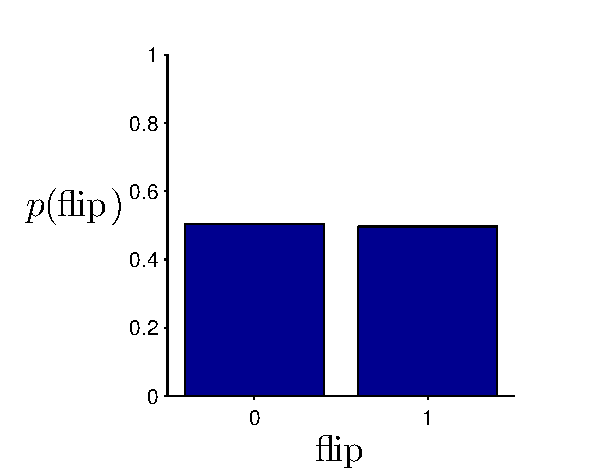
\includegraphics[width=0.45\textwidth]{figures/flipmarg}}
  \only<3>{
	  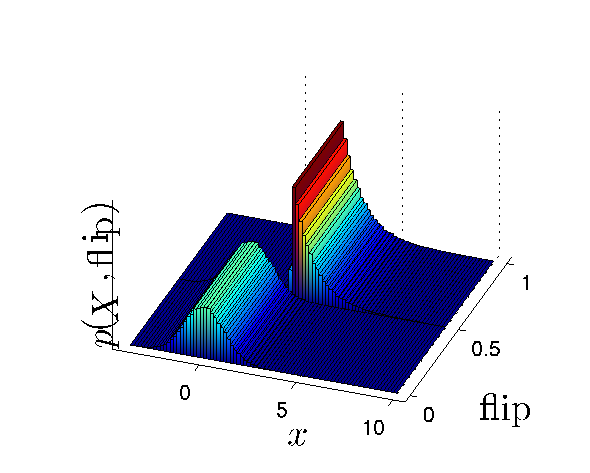
\includegraphics[width=0.45\textwidth]{figures/joint}
	  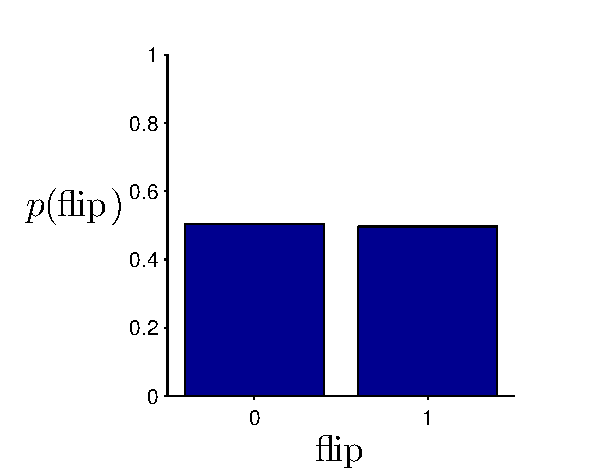
\includegraphics[width=0.45\textwidth]{figures/flipmarg}}
  \end{block}
\end{frame}

\begin{frame}{Probabilistic Programming: Conditioning}
%\TBD{DD}
%\TBD{Move this between earlier slides if sensible}
  \begin{block}{Once we've defined a prior, what can we do with it?}  

  The stochastic program defines joint distribution $P(D,N,H)$
  \begin{itemize}
    \item D to be the subset of variables we observe (condition on)
    \item H the set of variables we're interested in
    \item N the set of variables that we're not interested in, (so we'll integrate them out).
  \end{itemize}
  We want to know about $P(H|D)$
  \end{block}
  \begin{block}{Probabilistic Programming}
      \begin{itemize}
        \item Usually refers to doing conditionial inference when a probabilistic program specifies your prior.
      \end{itemize}
    \end{block}
\end{frame}

\begin{frame}{An Example Probabilistic Program: Conditioning}

%\begin{alltt}
\begin{lstlisting}[language=Matlab]
flip = rand < 0.5
if flip
    x = randg + 2   % Random draw from Gamma(1,1)
else
    x = randn       % Random draw from standard Normal
end
\end{lstlisting}
%\end{alltt}

  \begin{block}{Implied distributions over variables}

  %\begin{figure}
  \only<1>{
	  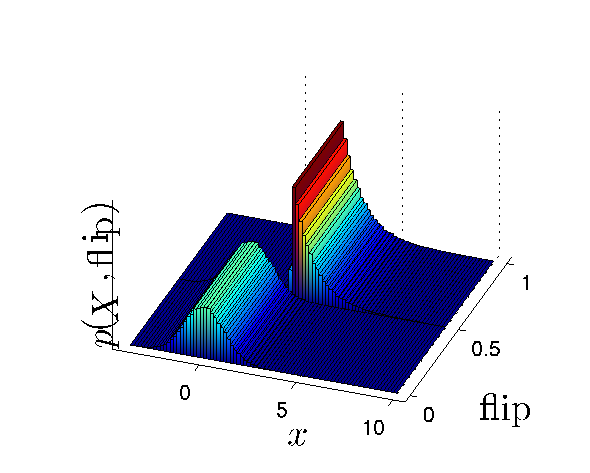
\includegraphics[width=0.45\textwidth]{figures/joint}
	  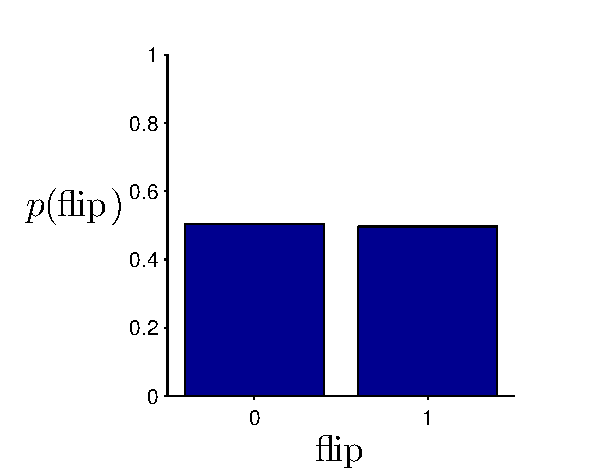
\includegraphics[width=0.45\textwidth]{figures/flipmarg}}
  \only<2>{
	  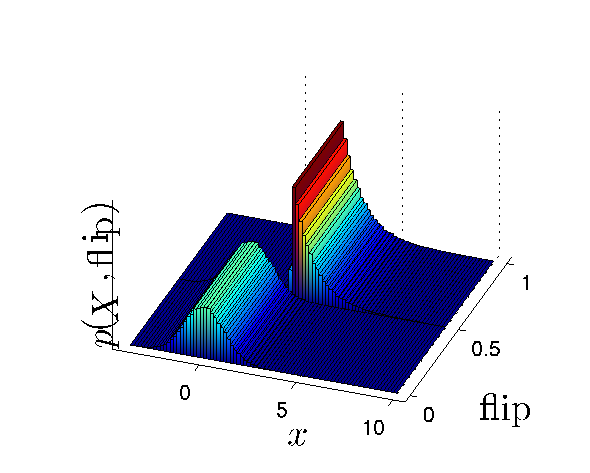
\includegraphics[width=0.45\textwidth]{figures/joint}
	  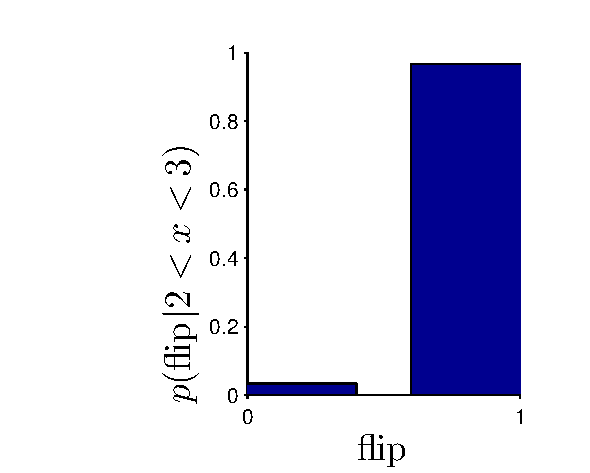
\includegraphics[width=0.45\textwidth]{figures/flipcond}}
  \end{block}
\end{frame}

\begin{frame}{Can we develop generic inference for all PPs?}
  \begin{block}{Rejection sampling}
    \begin{enumerate}
      \item Run the program with a fresh source of random numbers
      \item If condition $D$ is true, record $H$ as a sample, else ignore the sample
      \item Repeat
    \end{enumerate}
  \end{block}
  \begin{block}{Example}
    %\vspace{0.5\baselineskip}
    %\centering
    %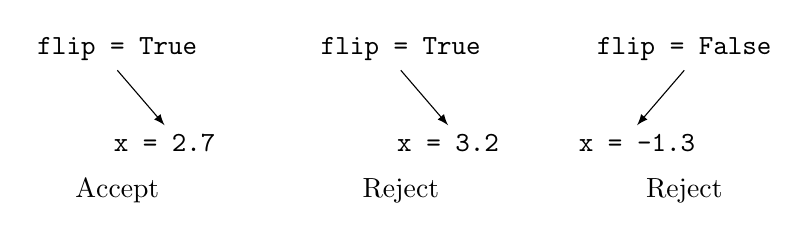
\begin{tikzpicture}[->,>=stealth',scale=1.2] 
  \begin{scope}[xshift=-3cm]
    \node[mybox] (root) at (0,0) {\texttt{flip = True}};
    \node[mybox] (left) at (-0.5,-1) {};
    \node[mybox] (right) at (0.5,-1) {\texttt{x = 2.7}};
    %\draw[-latex] (root.south) -- (left.north);
    \draw[-latex] (root.south) -- (right.north);
    \node[mybox] at (0,-1.5) {Accept};
  \end{scope}
  \begin{scope}[xshift=-0cm]
    \node[mybox] (root) at (0,0) {\texttt{flip = True}};
    \node[mybox] (left) at (-0.5,-1) {};
    \node[mybox] (right) at (0.5,-1) {\texttt{x = 3.2}};
    %\draw[-latex] (root.south) -- (left.north);
    \draw[-latex] (root.south) -- (right.north);
    \node[mybox] at (0,-1.5) {Reject};
  \end{scope}
  \begin{scope}[xshift=+3cm]
    \node[mybox] (root) at (0,0) {\texttt{flip = False}};
    \node[mybox] (left) at (-0.5,-1) {\texttt{x = -1.3}};
    \node[mybox] (right) at (0.5,-1) {};
    \draw[-latex] (root.south) -- (left.north);
    %\draw[-latex] (root.south) -- (right.north);
    \node[mybox] at (0,-1.5) {Reject};
  \end{scope}
\end{tikzpicture}

    \begin{columns}
      \begin{column}{.4\textwidth}
        \begin{alltt}
flip = rand < 0.5
if flip
\ \ x = randg + 2
else
\ \ x = randn
end
\end{alltt}

      \end{column}
      \begin{column}{.4\textwidth}
        
        \only<1>{
        \begin{alltt}
	        \
	        
	        \ 
	        
	        \ 
	        
	        \
	        
	        \
	        
	        \

        \end{alltt}
        }
        \only<2>{
        \begin{alltt}
	        >>True
	        
	        \ 
	        
	        \ 
	        
	        \
	        
	        \
	        
	        \

        \end{alltt}
        }
        \only<3>{
        \begin{alltt}
	        >>True
	        
	        \ 
	        
	        >>2.7
	        
	        \
	        
	        \
	        
	        \

        \end{alltt}
        }
        \only<4>{
        \begin{alltt}
	        \
	        
	        \ 
	        
	        \ 
	        
	        \
	        
	        \
	        
	        \

        \end{alltt}
        }
        \only<5>{
        \begin{alltt}
	        >>True
	        
	        \ 
	        
	        \ 
	        
	        \
	        
	        \
	        
	        \

        \end{alltt}
        }
        \only<6>{
        \begin{alltt}
	        >>True
	        
	        \ 
	        
	        >>3.2
	        
	        \
	        
	        \
	        
	        \

        \end{alltt}
        }
        \only<7>{
        \begin{alltt}
	        \
	        
	        \ 
	        
	        \ 
	        
	        \
	        
	        \
	        
	        \

        \end{alltt}
        }
        \only<8>{
        \begin{alltt}
	        >>True
	        
	        \ 
	        
	        \ 
	        
	        \
	        
	        \
	        
	        \

        \end{alltt}
        }
        \only<9>{
        \begin{alltt}
	        >>True
	        
	        \ 
	        
	        >>2.1
	        
	        \
	        
	        \
	        
	        \

        \end{alltt}
        }
        \only<10>{
        \begin{alltt}
	        \
	        
	        \ 
	        
	        \ 
	        
	        \
	        
	        \
	        
	        \

        \end{alltt}
        }
        \only<11>{
        \begin{alltt}
	        >>False
	        
	        \ 
	        
	        \ 
	        
	        \
	        
	        \
	        
	        \

        \end{alltt}
        }
        \only<12>{
        \begin{alltt}
	        >>False
	        
	        \ 
	        
	        \
	        
	        \
	        
	        >>-1.3
	        
	        \

        \end{alltt}
        }
        \only<13>{
        \begin{alltt}
	        \
	        
	        \ 
	        
	        \ 
	        
	        \
	        
	        \
	        
	        \

        \end{alltt}
        }
        \only<14>{
        \begin{alltt}
	        >>False
	        
	        \ 
	        
	        \ 
	        
	        \
	        
	        \
	        
	        \

        \end{alltt}
        }
        \only<15>{
        \begin{alltt}
	        >>False
	        
	        \ 
	        
	        \
	        
	        \
	        
	        >>2.3
	        
	        \

        \end{alltt}
        }

      \end{column}
    \end{columns}
  \end{block}
  \begin{block}{This produces samples over the \emph{execution trace}}
    \eg 
    \onslide<3->{\texttt{(True, 2.7)},}
    \onslide<9->{\texttt{(True, 2.1)},}
    \onslide<15->{\texttt{(False, 2.3)}, \dots}
  \end{block}
\end{frame}

\begin{frame}{Can we be more efficient?}
  \begin{block}{Metropolis-Hastings}
    \begin{enumerate}
  \onslide<1->{
    \item Start with a trace
    \begin{itemize}
      \item \texttt{(True, 2.3)}
    \end{itemize}
  }
  \onslide<2->{
    \item Change one random decision, discarding subsequent decisions
    \begin{itemize}
      \item \texttt{(False,)}
    \end{itemize}
  }
  \onslide<3->{
    \item Sample subsequent decisions
    \begin{itemize}
      \item \texttt{(False, -0.9)}
    \end{itemize}
  }
  \onslide<4->{
    \item Accept with appropriate (RJ)MCMC acceptance probability
    \begin{itemize}
      \item Reject, does not satisfy observation (\ie likelihood is zero)
    \end{itemize}
  }
\end{enumerate}

  \end{block}
\end{frame}

\begin{frame}{Can we be more efficient?}
  \begin{block}{Metropolis-Hastings}
    \begin{enumerate}
  \onslide<1->{
    \item Start with a trace
    \begin{itemize}
      \item \texttt{(True, 2.3)}
    \end{itemize}
  }
  \onslide<2->{
    \item Change one random decision, discarding subsequent decisions
    \begin{itemize}
      \item \texttt{(True, 2.9)}
    \end{itemize}
  }
  \onslide<3->{
    \item Sample subsequent decisions
    \begin{itemize}
      \item Nothing to do
    \end{itemize}
  }
  \onslide<4->{
    \item Accept with appropriate (RJ)MCMC acceptance probability
    \begin{itemize}
      \item Accept, maybe
    \end{itemize}
  }
\end{enumerate}

  \end{block}
\end{frame}

\begin{frame}{PP via Metropolis-Hastings - notation}
  \begin{block}{}
    %Following Wingate et alia \TBD{ref} we represent an unconditioned PP as a parameterless random function $f$ (or as a deterministic function which takes a source of randomness as an input)
    %\newline
    %
    Evaluating a program results in a sequence of random choices
    \begin{equation*}
      x_k \sim p_{t_k}(.|\theta_{k},x_1,\ldots,x_{k-1}).
    \end{equation*}
    where $\theta_{k}$ represents parameters of the distribution not included in $(x_1,\ldots,x_{k-1})$.
    \newline
    
    The density / probability of a particular evaluation is then
    \begin{equation*}
      p(x_1,\ldots,x_K) = \prod_{k=1}^K p_{t_k}(x_k|\theta_{k},x_1,\ldots,x_{k-1}).
    \end{equation*}
    
    We then perform MH over the the execution trace $x = (x_1,\ldots,x_K)$.
    
  \end{block}
\end{frame}

\begin{frame}{MH over execution traces}
  \begin{enumerate}
    \item Select a random decision in the execution trace $x$
    \begin{itemize}
      \item{\eg $x_k$}
    \end{itemize}
    \vspace{\baselineskip}
    \item Propose a new value
    \begin{itemize}
      \item{\eg $x_k' \sim K_{t_k}(.|x_k,\theta_k)$}
    \end{itemize}
    \vspace{\baselineskip}
    \item Run the program to determine all subsequent choices $(x_l' : l > k)$, reusing current choices where possible
    \vspace{\baselineskip}
    \item Propose moving from the state $(x_1,\ldots,x_K)$ to $(x_1,\ldots,x_{k-1},x_k',\ldots,x_{K'}')$
    \vspace{\baselineskip}
    \item Accept the change with the appropriate MH acceptance probability
  \end{enumerate}
  \begin{equation*}
    \frac{K_{t_k}(x_k|x_k',\theta_k)\prod_{i=k}^{K'} p_{t_i'}(x_i'|\theta_{i}',x_1,\ldots,x_{k-1},x_k',\ldots,x_{i-1}')}{K_{t_k}(x_k'|x_k,\theta_k)\prod_{i=k}^K p_{t_i}(x_i|\theta_{i},x_1,\ldots,x_{i-1})}
  \end{equation*}
\end{frame}

%\begin{frame}{Worked example}
%\TBD{If there is time}
%\end{frame}

\begin{frame}{Advanced Automatic Inference}

    \begin{itemize}
      \item Now that we have separated inference and model design, can use any inference algorithm.
      \item Free to develop inference algorithms independently of specific models.
      \item Once graphical models identified as a general class, many model-agnostic inference methods:
      \begin{itemize}
	      \item Belief Propagation
	      \item Pseudo-likelihood
	      \item Mean-field Variational
	      \item MCMC
	    \end{itemize}
    \item What generic inference algorithms can we implement for more expressive generative models?
    \end{itemize}
\end{frame}


\begin{frame}{Advanced Automatic Inference: Gibbs}
    \begin{itemize}
      \item BUGS: {\bf B}ayesian inference {\bf U}sing {\bf G}ibbs {\bf S}ampling
        \begin{itemize}
      \item An early, limited form of automated inference in generative models.
      \item Began in 1989 in the MRC Biostatistics Unit, Cambridge, UK.
      \item A workhorse of applied statisticians.  Also JAGS (open-source)
    \end{itemize}
    \end{itemize}
    
\begin{alltt}
{\tiny
model\{	
  for( i in 1 : N ) \{
    S[i] ~ dcat(pi[])
    mu[i] <- theta[S[i]]
    x[i] ~ dpois(mu[i])	
    for (j in 1 : C) \{
      SC[i, j] <- equals(j, S[i])\}\}
    # Precision Parameter 		
    alpha~ dgamma(0.1,0.1)
    # Constructive DPP
    p[1] <- r[1]
    for (j in 2 : C) \{
      p[j] <- r[j] * (1 - r[j - 1]) * p[j -1 ] / r[j - 1]\}
    p.sum <- sum(p[])		
    for (j in 1:C)\{     
      theta[j] ~ dgamma(A, B)
      r[j] ~ dbeta(1, alpha)			
      # scaling to ensure sum to 1 
      pi[j] <- p[j] / p.sum \}
    # hierarchical prior on theta[i] or preset parameters
    A ~ dexp(0.1)     B ~dgamma(0.1, 0.1)
    # total clusters			
    K <- sum(cl[])
    for (j in 1 : C) \{
      sumSC[j] <- sum(SC[ , j])
      cl[j] <- step(sumSC[j] -1)\}\}

Data:
list(x=c(0,0,0,0,0,0,0,0,0,0,0,0,0,0,0,0,0,0,0,0,0,0,0,0,0,0,0,0,0,0,0,0,
0,0,0,0,0,0,0,0,0,0,0,0,0,0,1,1,1,1,1,1,1,1,1,1,1,1,1,1,2,2,2,2,2,2,2,2,
2,3, 3, 3, 3, 4, 4, 5, 5, 5, 6, 6, 6,7,7,7,8,9,9,10, 10,
11, 11, 12,  12,  14,  15,  15,  17,  17,  22,  24,  34), N=101, C=19)

Results
node        mean   sd      MC error 2.5\%   median  97.5\%  start   sample
Deviance    301.3  15.86   0.4314   269.3   301.7   332.2   1001    10000
K           6.764  1.494   0.07225  4.0	7.0 10.0    1001    10000
mu[92]      13.34  3.113   0.04068  5.656   14.11   17.5    1001    10000}
\end{alltt}    

\end{frame}

%\begin{frame}{Advanced Automatic Inference: Exact}
%    \begin{itemize}
%      \item Cosh (exhaustive enumeration)
%      \item Stuhlmueller's recent work
%      \item Wingate's enumeration
%    \end{itemize}
%\end{frame}

\begin{frame}{Advanced Automatic Inference: Metropolis-Hastings}
    \begin{itemize}
      \item Bher, MIT-Church
      \\ {\color{DarkBlue}(Goodman, Mansinghka, Roy, Bonawitz and Tenenbaum, 2008)}
      \begin{itemize}
         \item (Automatic inference in Scheme)
      \end{itemize}      
      \item Stochastic Matlab
    \begin{itemize}
      \item Lightweight Implementations of Probabilistic Programming Languages Via Transformational Compilation {\color{DarkBlue} 
      
      (Wingate, Stuhlm\"{u}ller, Goodman, 2011)}
    \end{itemize}      
            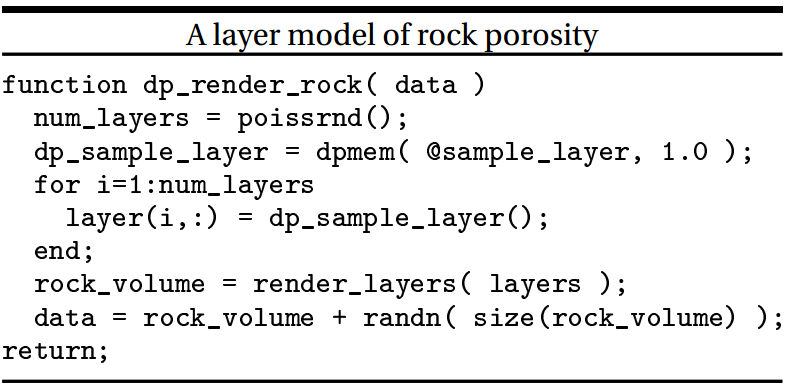
\includegraphics[width=5.5cm]{figures/probmatlab.png}
            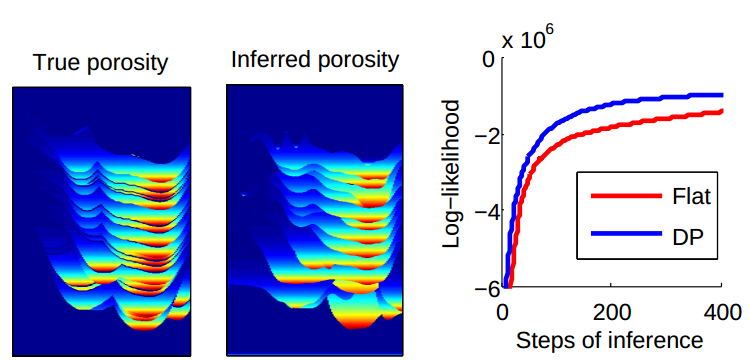
\includegraphics[width=5.5cm]{figures/probmatlab2.png}
    \end{itemize}
\end{frame}

\begin{frame}{Advanced Automatic Inference: HMC}

    \begin{itemize}
      \item Automatic Differentiation in Church:
      \\ Nonstandard Interpretations of Probabilistic Programs for Efficient Inference
{\color{DarkBlue} (Wingate, Goodman, Stuhlmuller, Siskind, 2012)}
      \item Stan (Gelman et al)
      \\
      \texttt{http://mc-stan.org/}
      \begin{alltt}
{\tiny
// Predict from Gaussian Process Logistic Regression
// Fixed covar function: eta_sq=1, rho_sq=1, sigma_sq=0.1

data \{
  int<lower=1> N1;     
  vector[N1] x1; 
  int<lower=0,upper=1> z1[N1];
  int<lower=1> N2;
  vector[N2] x2;\}
transformed data \{
  int<lower=1> N;
  vector[N1+N2] x;
  vector[N1+N2] mu;
  cov_matrix[N1+N2] Sigma;
  N <- N1 + N2;
  for (n in 1:N1) x[n] <- x1[n];
  for (n in 1:N2) x[N1 + n] <- x2[n];
  for (i in 1:N) mu[i] <- 0;
  for (i in 1:N) 
    for (j in 1:N)
      Sigma[i,j] <- exp(-pow(x[i] - x[j],2))
                    + if_else(i==j, 0.1, 0.0);\}
parameters \{
  vector[N1] y1;
  vector[N2] y2;\}
model \{
  vector[N] y;
  for (n in 1:N1) y[n] <- y1[n];
  for (n in 1:N2) y[N1 + n] <- y2[n];

  y ~ multi_normal(mu,Sigma);
  for (n in 1:N1)
    z1[n] ~ bernoulli_logit(y1[n]);\}}
\end{alltt}  
      
    \end{itemize}

\end{frame}

\begin{frame}{Advanced Automatic Inference: Expectation Propagation}
    \begin{itemize}
      \item Infer.NET {\color{DarkBlue} (Minka, Winn, Guiver, Knowles, 2012)}
      \begin{itemize}
        \item EP in graphical models:
        \item Now works in functional language F\#:
        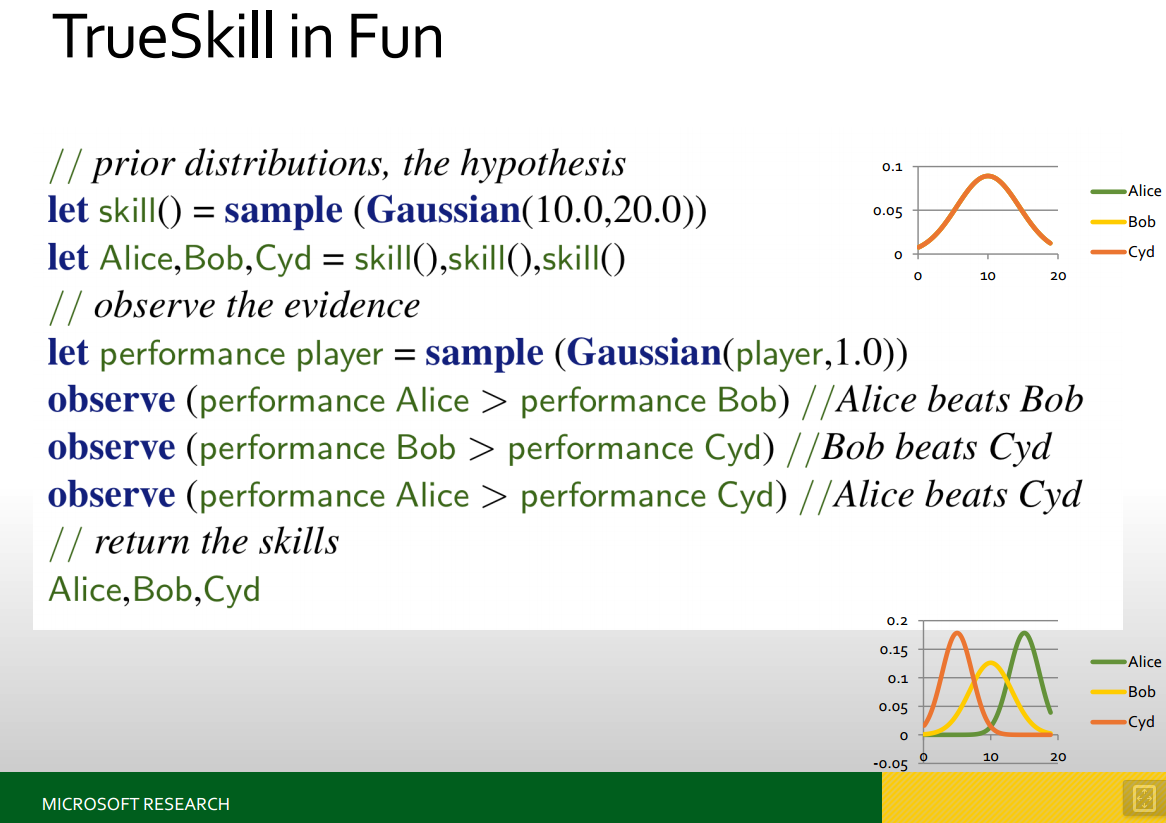
\includegraphics[width=8cm]{figures/fun}
      \end{itemize}
    \end{itemize}
    
\end{frame}

\begin{frame}{Advanced Automatic Inference: Variational}

    \begin{itemize}
      \item Infer.NET has it too.
      \item Automated Variational Inference in Probabilistic Programming
      \\ {\color{DarkBlue}  (Wingate, Weber, 2012) }
      \\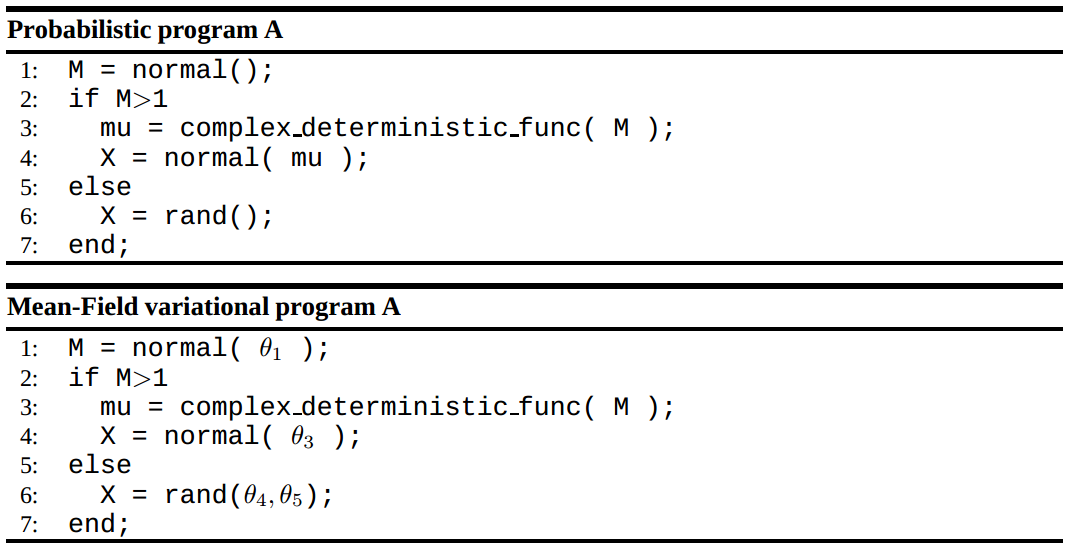
\includegraphics[width=8cm]{figures/meanvar}
      \item Learning phase: Forward sample, then stochastically update $\theta$s to minimize expected KL from true distribution.
      \item Dependency of variatonal dist on control logic remains.
    \end{itemize}

\end{frame}


\begin{frame}{Advanced Automatic Inference: Hardware}
    \begin{itemize}
      \item Natively Probabilistic Computation {\color{DarkBlue}  (Mansinghka, 2009) }
      \item Lyric Semiconductor? (Error correcting codes)
      \item Main idea: If we know we're going to be sampling, might as well take advantage of thermal noise in our hardware.
          \begin{itemize}
                \item Samplers can be made robust to computational error.
                \item Run at low voltage on (cheap?) FPGA
          \end{itemize}        
      \item Compile from generative model to FPGA (9x9 Ising model sampler):
      \\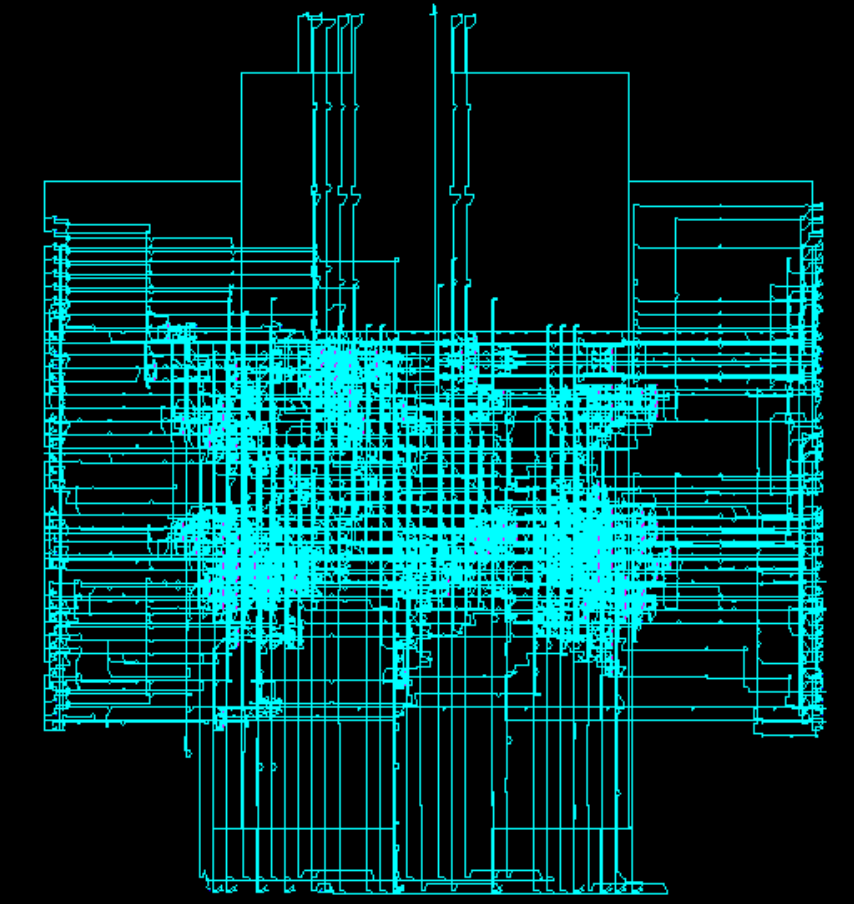
\includegraphics[width=5cm]{figures/llvm}
    \end{itemize}
\end{frame}

%\begin{frame}{Main strength}
%\TBD{Dave}
%Writing non-parametric models easy

%Only need to evaluate samples from non-parametric objext lazily
%\end{frame}

\begin{frame}{Nonparametric models}
  \begin{itemize}
    \item If we can sample from the prior of a nonparametric model using finite resources with probability 1, then we can apply probabilistic programming
    \vspace{\baselineskip}
    \item This can be achieved for a number of nonparametric processes/models \eg
    \begin{itemize}
      \item Marginalisation (\eg Gaussian process)
      \item Stick breaking (\eg Dirichlet process)
      \item Urn scheme (\eg Indian Buffet process)\dots
    \end{itemize}
    \vspace{\baselineskip}
    \item Active research to produce finite sampling algorithms for other nonparametric processes (\eg hierarchical beta processes, negative binomial process \TBD{cite Koa and Dan})
  \end{itemize}
\end{frame}



\begin{frame}{Example: Mixture of Gaussians}
  \begin{columns}
    \begin{column}{.47\textwidth}
      \begin{block}{Generative model}
        \begin{eqnarray*}
          (\mu_k)_{k=1\ldots K} & \simiid & \mathcal{N}(0, 1) \\
          (\pi_k)_{k=1\ldots K} & \sim & \textrm{Dir}(\alpha/K) \\
          \Theta & := & \sum_{k=1}^K \pi_k \delta_{\mu_k} \\
          (\theta_n)_{n=1\ldots N} & \simiid & \Theta \\
          (x_i)_{n=1\ldots N} & \sim & \mathcal{N}(\theta_n, 1)
        \end{eqnarray*}
      \end{block}
    \end{column}
    \begin{column}{.47\textwidth}
      \begin{block}{(Pseudo) MATLAB code}
        \vspace{0.75\baselineskip}
        \begin{alltt}
          mu = randn(K,1)

          pi = dirichlet(K, alpha/K)

          for n = 1:N
            
          \ \ theta = mu(mnrnd(1,pi))
          
          \ \ x(n) \ = theta + randn
            
          end
        \end{alltt}
        \vspace{0.75\baselineskip}
      \end{block}
    \end{column}
  \end{columns}
  \vspace{\baselineskip}
  \begin{center}
  {
    {Note that the pseudo-code makes the potentially ambiguous\\conditional independence structure transparent}
  }	
  \end{center}
  \vspace{-1\baselineskip}
\end{frame}

\begin{frame}{Example: Infinite mixture of Gaussians}
  \begin{block}{Change to generative model}
    \begin{eqnarray*}
      (\mu_i)_{i=1\ldots k} \simiid \mathcal{N}(0, 1) &\\
      (\pi_i)_{i=1\ldots k} \sim \textrm{Dir}(\alpha/k) & \\
      \Theta := \sum_{i=1}^k \pi_i \delta_{\mu_i} & \underset{k \to \infty}{\to} & \Theta \sim \textrm{DP}(\alpha, \mathcal{N}(0,1))
    \end{eqnarray*}
  \end{block}
  \begin{block}{Avoiding infinity}
    \vspace{0.5\baselineskip}
    \begin{itemize}
      \item $\Theta$ is now infinitely complex, and can only be represented approximately with finite resources
      \vspace{0.5\baselineskip}
      \item However, we can sample a finite number of samples $(\theta_i)_{i=1\ldots n}$ from some unknown $\Theta$ in finite time (with probability 1) using a stick breaking algorithm
    \end{itemize}
  \end{block}
\end{frame}  

\begin{frame}{Example: Infinite mixture of Gaussians}
  \begin{block}{(Pseudo) MATLAB code - stick breaking construction}
    \begin{alltt}
      sticks = [];
      
      atoms = [];
      
      
      for i = 1:n
      
      \ \ p = rand;
      
      \ \ while p > sum(sticks)
      
      \ \ \ \ sticks(end+1) = (1-sum(sticks)) * betarnd(1, alpha);
      
      \ \ \ \ atoms(end+1) \ = randn;
      
      \ \ end
      
      \ \ theta(i) = atoms(find(cumsum(sticks)>=p, 1, `first'));
      
      end
      
      
      x = theta' + randn(n, 1);
    \end{alltt}
  \end{block}
\end{frame}

\begin{frame}{Stochastic memoisation}
  \TBD{Probably delete unless I can find a nice way to say this}
  \begin{itemize}
    \item Stick breaking considered useful enough to be a language construction \TBD{Correct language?} in Church
    \vspace{\baselineskip}
    \item A random parameterless function $P$ can be stochastically memoised
    \begin{itemize}
      \item Mathematically equivalent to $P \to \textrm{DP}(\alpha, P)$
    \end{itemize}
    \vspace{\baselineskip}
    \item Called stochastic memoisation since the base function $P$ is called only occasionally with old return values being recycled on some calls
    \vspace{\baselineskip}
    \item Implemented via stick breaking \TBD{Is this true?}
    \vspace{\baselineskip}
    \item Latest descendant of Church (Venture) has a CRP construction which allows DP like behaviour when used in conjunction with normal memoisation
  \end{itemize}
\end{frame}

\begin{frame}{Demos}

\end{frame}


\begin{frame}{Compiler Development}
  \begin{itemize}
    \item 1950s: Ask a programmer to implement an algorithm efficiently:  They'll write it on their own in assembly.
    \begin{itemize}
      \item No good compilers; problem-dependent optimizations that only human expert could see.
    \end{itemize}
    \vspace{\baselineskip}
    \item 1970s: Novice programmers use high-level languages and let compiler work out details, experts still write assembly.
    \begin{itemize}
      \item Experts still write custom assembly when speed critical.
    \end{itemize}
    \vspace{\baselineskip}
    \item 2000s: On most problems, even experts can't write faster assembly than optimizing compilers.
    \begin{itemize}
      \item can automatically profile (JIT).
      \item can take advantage of paralellization, complicated hardware, make appropriate choices w.r.t. caching.
      \item Compilers embody decades of compiler research
    \end{itemize}    
    \vspace{\baselineskip}
  \end{itemize}
\end{frame}


\begin{frame}{Inference Methods in the Future}
  \begin{itemize}
    \item 2010: Ask a grad student to implement inference efficiently:  They'll write it on their own.
    \begin{itemize}
      \item No good automatic inference engines; problem-dependent optimizations that only human expert can see.
    \end{itemize}
    \vspace{\baselineskip}
    \item 2015: Novice grad students use automatic inference engines and let compiler work out details, experts still write their own inference.
    \begin{itemize}
      \item Experts still write custom inference when speed critical.
    \end{itemize}
    \vspace{\baselineskip}
    \item 2020: On most problems, even experts can't write faster inference than mature automatic inference engines.
    \begin{itemize}
      \item Can use paralellization, sophisticated hardware
      \item Can automatically choose appropriate methods (meta-reasoning?).
      \item Inference engines will embody 1 decade (!) of PP research.
    \end{itemize}    
    \vspace{\baselineskip}
  \end{itemize}
\end{frame}


\begin{frame}{How to write a Bayesian modeling paper: 2010}
  \begin{block}{}
    \begin{enumerate}
      \item Write down a generative model in an afternoon
      \vspace{\baselineskip}
      \vspace{\baselineskip}
      \item Get 2 grad students to implement inference for a month
      \vspace{\baselineskip}
      \vspace{\baselineskip}
      \item Use technical details of inference to pad half of the paper
    \end{enumerate}
  \end{block}
\end{frame}

\begin{frame}{How to write a Bayesian modeling paper: 2020}
  \begin{block}{}
    \begin{enumerate}
      \item Write down a generative model in an afternoon
      \vspace{\baselineskip}
      \vspace{\baselineskip}
      \item \sout{Get 2 grad students to implement inference for a month} 
      \\ Run automatic inference engine.
      \vspace{\baselineskip}
      \vspace{\baselineskip}
      \item Use technical details of inference to pad half of the paper
    \end{enumerate}
  \end{block}
\end{frame}

\begin{frame}{How to write a Bayesian modeling paper: 2020}
  \begin{block}{}
    \begin{enumerate}
      \item Write down a generative model in an afternoon
      \vspace{\baselineskip}
      \vspace{\baselineskip}
      \item \sout{Get 2 grad students to implement inference for a month} 
      \\Run automatic inference engine.
      \vspace{\baselineskip}
      \vspace{\baselineskip}
      \item \sout{Use technical details of inference to pad half of the paper}
      \\ Discuss strengths and weaknesses of the model in the extra 4 pages.
    \end{enumerate}
  \end{block}
\end{frame}


\end{document}


